\section{World and Machine}
The \emph{machine} is the portion of system to be developed (software and hardware).
The \emph{world} (aka the environment) is the portion of the real world affected by the machine.

Phenomena can be \emph{shared} between world and machine.
Shared phenomena can be controlled by the machine and observed by the world, or viceversa.

\textbf{Goals} are prescriptive assertions formulated in terms of world phenomena.\\
\textbf{Domain assumptions} are descriptive assertions assumed to hold in the world.\\
\textbf{Requirements} are prescriptive assertions formulated in terms of shared phenomena.

Example of interaction betweem world and machine:
\todo[inline]{make this bigger}
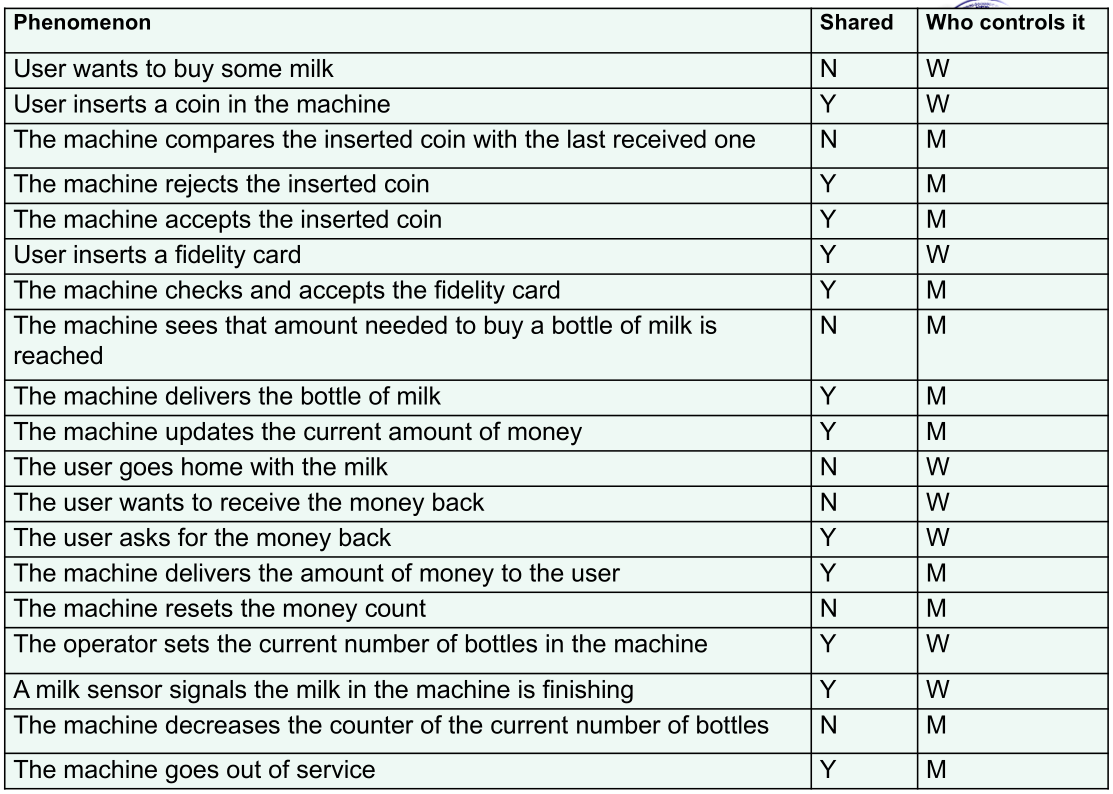
\includegraphics[width=\linewidth]{3-world-machine/shared-example.png}